\documentclass[tikz,border=10pt]{standalone}
\usepackage{amsmath}
\usepackage{tikz}
\usetikzlibrary{arrows.meta, angles, quotes}
\usetikzlibrary{decorations.markings,intersections,calc}
\usetikzlibrary{shapes}
\usepackage{amssymb}
\usepackage{physics}
\usepackage{bm}
\usepackage{xcolor}
\tikzset{omega_arrows/.style={-stealth,thin,draw=gray!60}}
\tikzset{L_vectors/.style={-stealth,very thick,red}}

% Parameter voor aantal pijlen dat er zal getekend worden
\def\NA{20}


% Parameters van het blok (h, w en d in cm)
\def\m{6}
\def\h{1}
\def\w{2}
\def\d{0.5}


\begin{document}
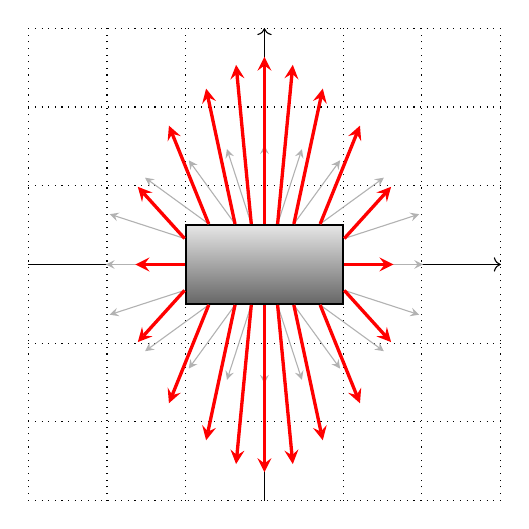
\begin{tikzpicture}

    %definieren assenstelsel voor de leesbaarheid
    \draw[thin,dotted] (-3,-3) grid (3,3);
    \draw[->] (-3,0) -- (3,0);
    \draw[->] (0,-3) -- (0,3);

    %Nu een poging voor een balk:

    \node (rectangle) at (0,0)   [draw, thick, rectangle, shade,  top color=black!10, bottom color=black!60, minimum width= \w cm, minimum height= \h cm,]{};

    % \foreach \i [evaluate={\angle=(\i-1)*360/\NA;}] in {1,...,\NA}
    %     {\draw[omega_arrows](rectangle.\angle) -- ++(\angle:1);}

    
    % --- Bereken de traagheidstensorcomponenten ---
    \pgfmathsetmacro{\Ixx}{1/12*\m*(\h^2+\d^2)}
    \pgfmathsetmacro{\Iyy}{1/12*\m*(\w^2+\d^2)}


    % --- For-loop over de hoeken ---
    \foreach \i [evaluate={\angle=(\i-1)*360/\NA;}] in {1,...,\NA}{
    % omega vector (lengte 1)
    \pgfmathsetmacro{\wx}{cos(\angle)}
    \pgfmathsetmacro{\wy}{sin(\angle)}

    % overeenkomstige L = I * omega
    \pgfmathsetmacro{\Lx}{\Ixx*\wx}
    \pgfmathsetmacro{\Ly}{\Iyy*\wy}

    % pijl voor omega
    \draw[omega_arrows]
      (rectangle.\angle) -- ++(\angle:1);

    % pijl voor L (zelfde aangrijpingspunt)
    \draw[L_vectors]
      (rectangle.\angle) -- ++({\Lx},{\Ly});}




    %Neem aan dat de balk width w (x-direction), height h (y-direction), depth d (z-direction) heeft en een massa m. De traagheidstensor wordt dan
    % I=[[1/12*m*(h**2+d**2),0,0],[0,1/12*m*(w**2+d**2),0],[0,0,1/12*m*(w**2+h**2)]]
    %We zijn dan geinteresseerd in vector L voor een zekere vector omega. Er geldt simpelweg dat L= dotproduct(I,omega). We gaan nu voor verschillende 
    %omega (allen norm één maar onder verschillende hoeken) de vector L berekenen en zowel omega in het lichtgrijs als L in het rood tekenen op de rand 
    %van de balk. Uiteraard zijn we, want het gaat om een 2D figuur, enkel geinteresseerd in vectoren in het XY vlak.










\end{tikzpicture}
\end{document}